
\documentclass[aspectratio=169]{beamer}
\setbeamertemplate{navigation symbols}{}

\usepackage{subfigure,epsfig,amsfonts}
\usepackage{beamerthemeshadow}
\usepackage{amsmath}
\usepackage{bm}

\setbeamertemplate{footline}{}
\setbeamertemplate{navigation symbols}{}

\begin{document}
\title{Stochastic computation in recurrent networks of spiking neurons}  
\author{Clayton Seitz}
\date{\today} 

\maketitle

\begin{frame}{The squid giant axon}

Hodkin and Huxley developed a mathematical model for nerve cell communication in 1952 using voltage data from the giant axon of a squid

\begin{figure}
\centering
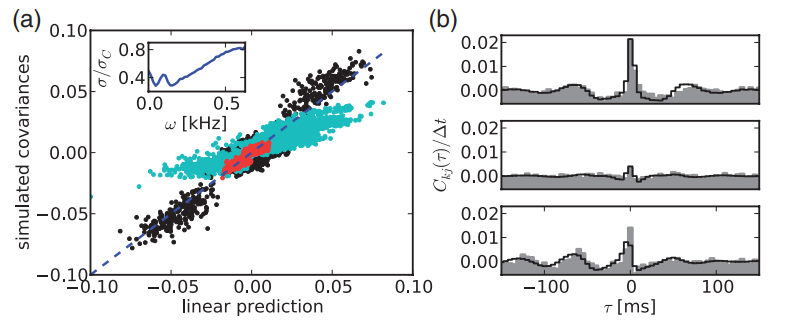
\includegraphics[width=95mm]{figure-20}
\end{figure}

\end{frame}

\begin{frame}{$Na^{+}$ and $K^{+}$ are the major charge carriers}

\begin{figure}
\centering
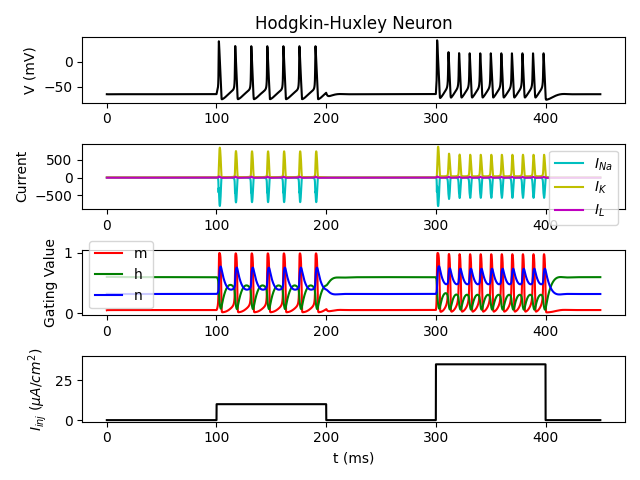
\includegraphics[width=105mm]{figure-19}
\end{figure}

\end{frame}

\begin{frame}{$Ca^{2+}$ sensors enable high-speed two-photon imaging}

Animal models and experimental technologies have improved drastically

Scale bars: b, 250 um; c, d, 100 um
\begin{figure}
\centering
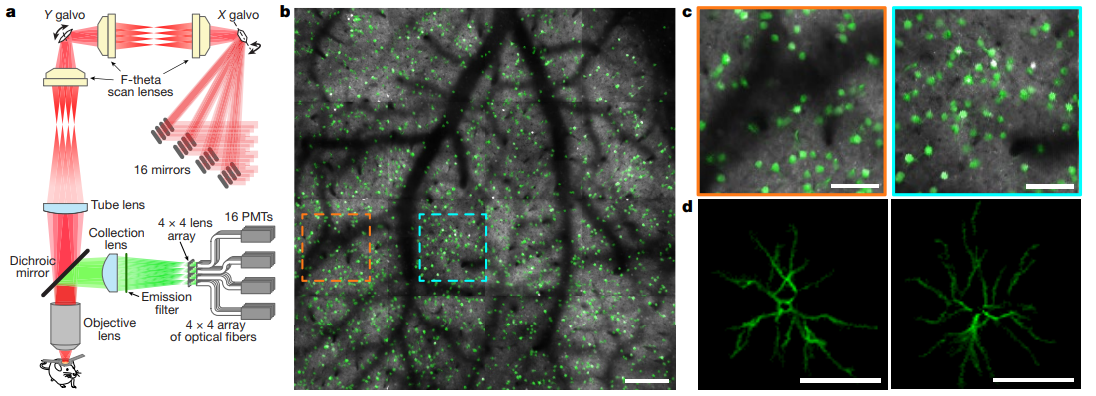
\includegraphics[width=140mm]{figure-16}
\end{figure}

But our mathematical and physical theories of sensory processing are lacking...

\end{frame}

\begin{frame}{Spiking neural networks: integrate and fire models}


\begin{figure}
\centering
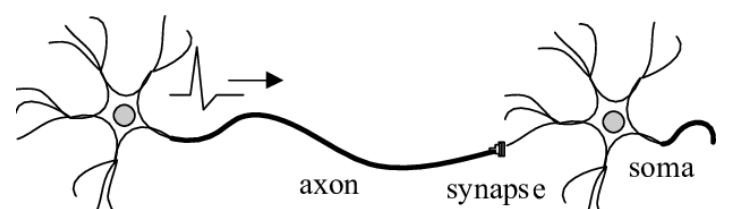
\includegraphics[width=75mm]{figure-15}
\end{figure}

\begin{figure}
\centering
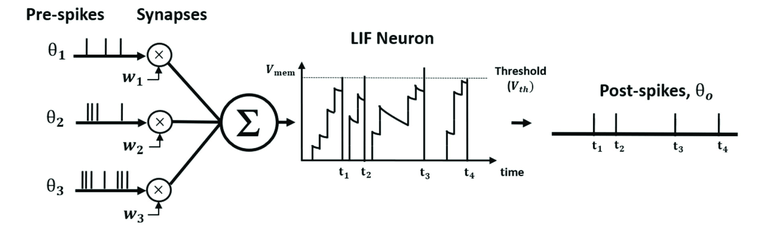
\includegraphics[width=125mm]{figure-14}
\end{figure}

\begin{equation*}
\tau\dot{V(t)} = -g_{L}V(t) + \sum_{n} w_{n}\theta_{n}(t)
\end{equation*}

\end{frame}


\begin{frame}{Synaptic strengths are dynamic}

$w_{n}$ represents the change in the post-synaptic membrane potential induced by an action potential at the presynaptic cell

\begin{figure}
\centering
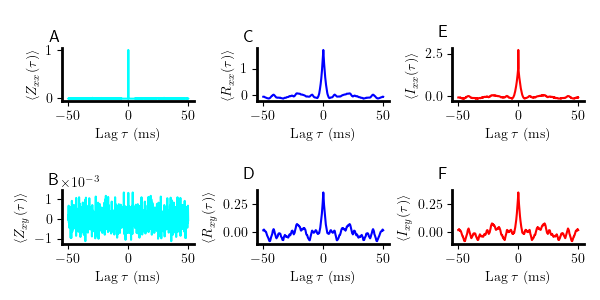
\includegraphics[width=95mm]{figure-12}
\end{figure}

$w_{n}$ is a result of complex biochemical pathways and is not necessarily a constant (synaptic plasticity)

\end{frame}

\begin{frame}{Langevin dynamics of the membrane potential}

\begin{figure}
\centering
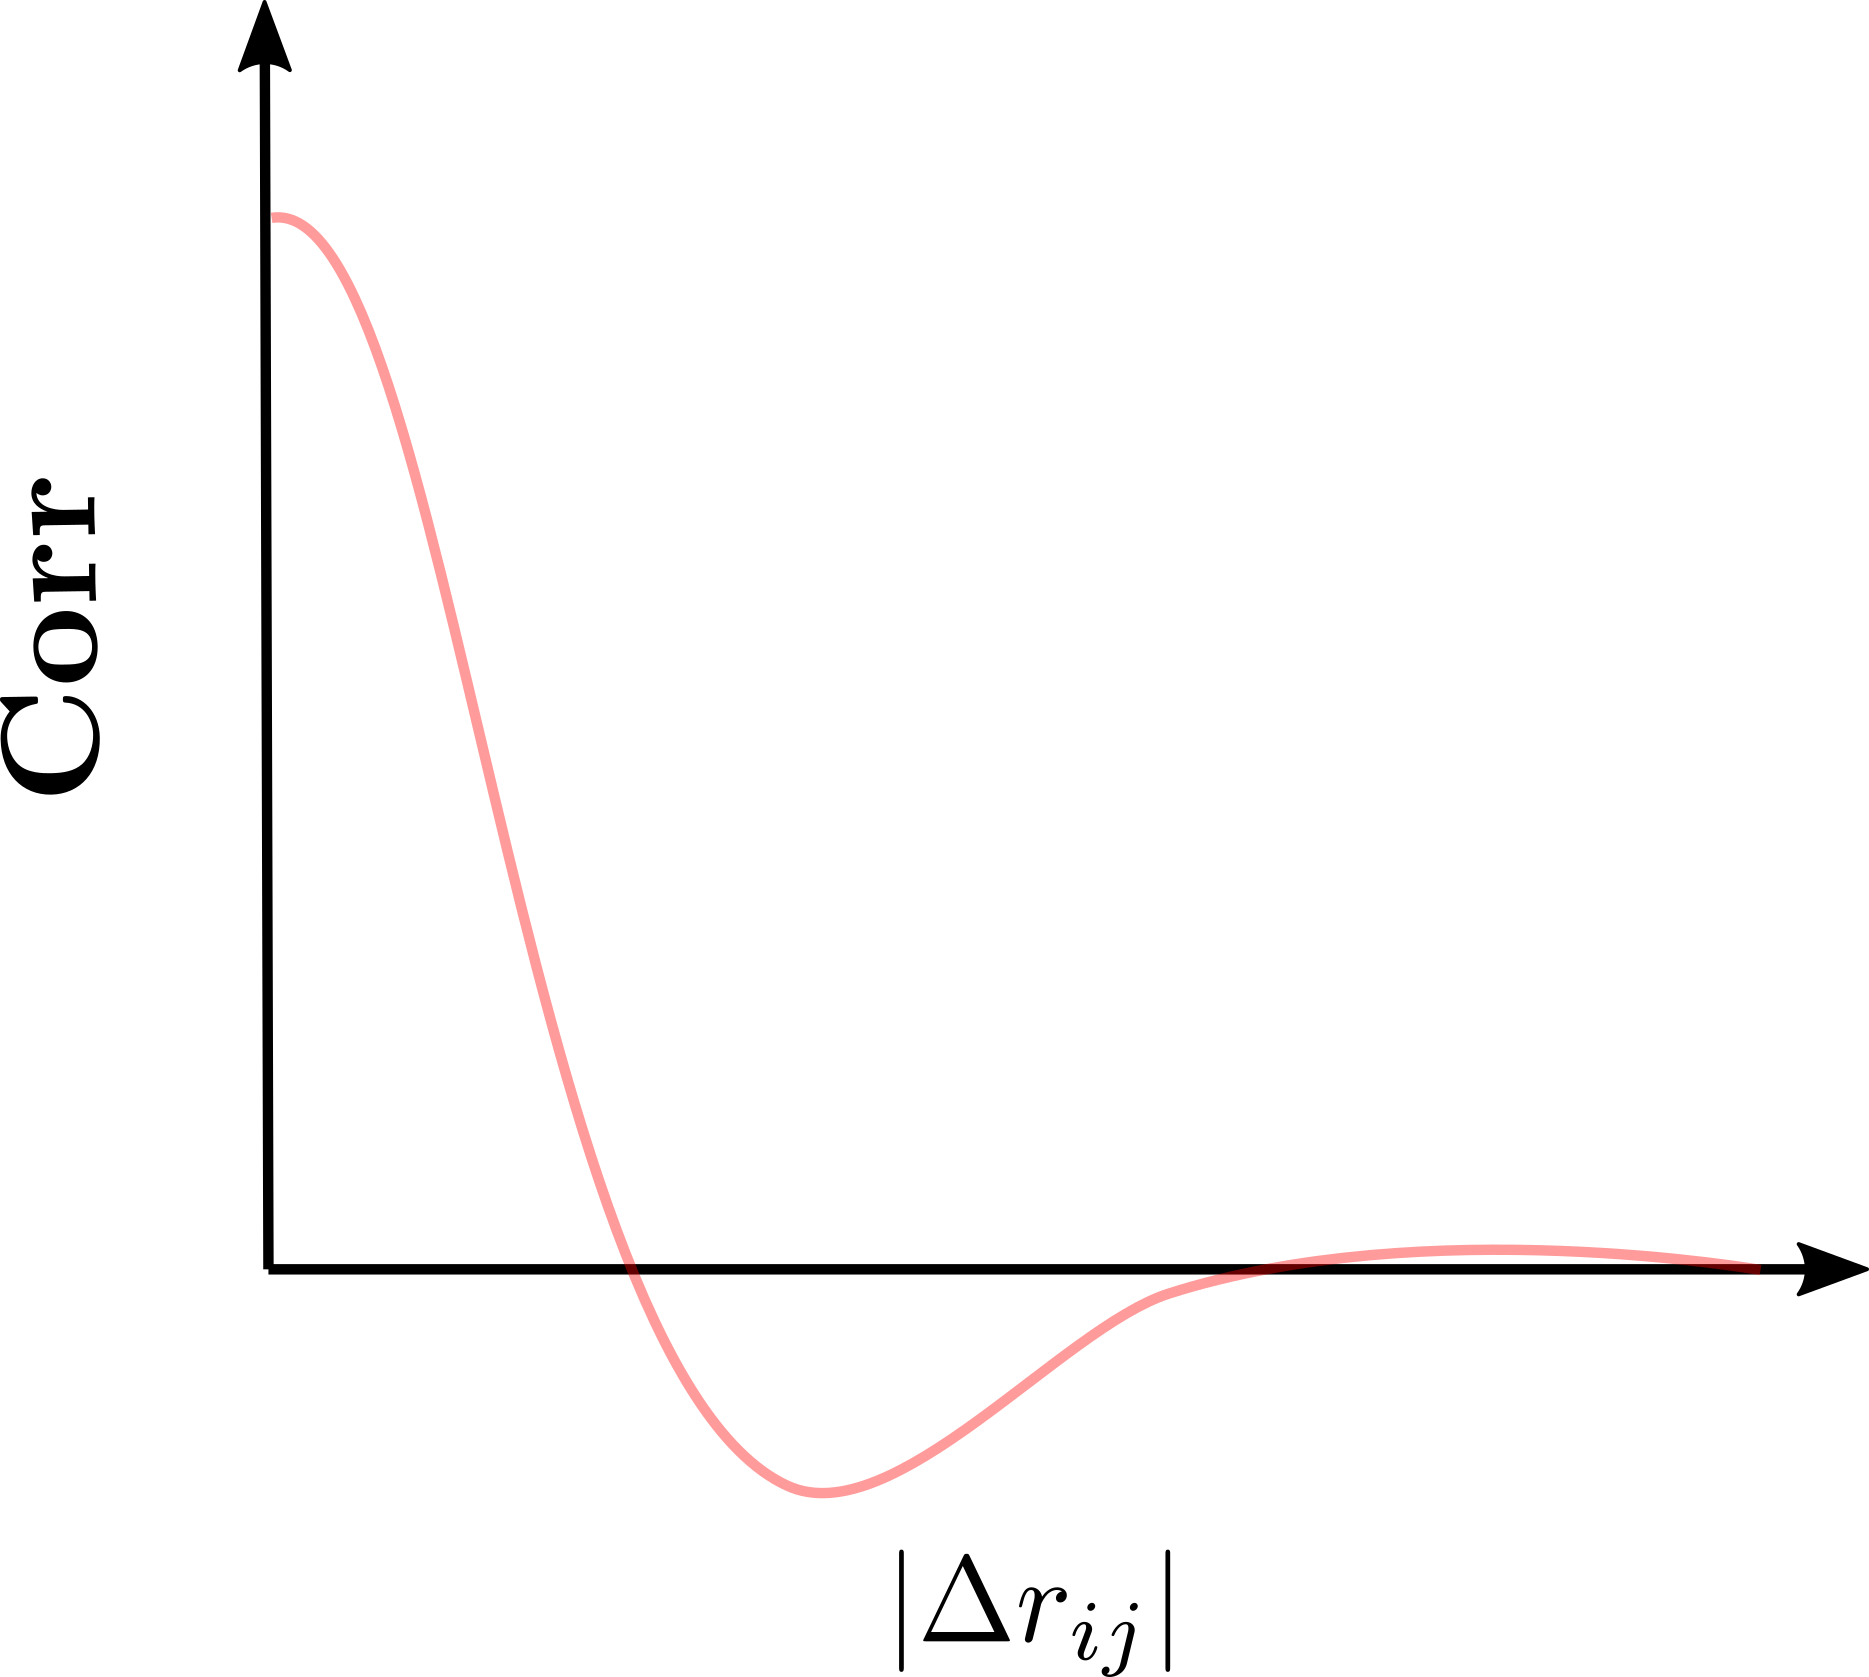
\includegraphics[width=100mm]{figure-10}
\end{figure}

Predicting $I(t)$ is hard especially with dynamic synapses. We often model $I(t)$ as a stochastic process e.g., $I(t) = \mu(t) + \sqrt{2D}\eta(t)$

\begin{equation*}
\tau\dot{V(t)} = -g_{L}V(t) + \mu(t) + \sqrt{2D}\eta(t)
\end{equation*}

which is a Langevin equation

\end{frame}

\begin{frame}{Statistical mechanics of networks of neurons}

\end{frame}


\end{document}